\secrel{Входная цепь\ --- фоторезистор (LDR)}

\begin{tabular}{p{0.62\textwidth} l}
\parbox[b]{0.62\textwidth}{
LDR\note{Light Dependent Resistor} или фоторезистор\ --- типичный компонент,
используемый в цепях измерения уровня освещенности. LDR изменяет сопротивление
пропорционально интенсивности света, падающего на него. Фоторезисторы
изготавливаются из полупроводников, таких как селен, оксид таллия и сульфид
кадмия. Когда фотоны света сталкиваются с атомами в материале LDR, проводимость
увеличивается, и электроны могут течь через цепь. Это означает, что по мере
увеличения уровня освещенности, сопротивление уменьшается.

\bigskip
Фоторезисторы можно использовать только с маленьким протекающим через него током
порядка 5\,мА, если превышается допустимый ток, LDR перегревается и сгорает.
Обычно они используются в схеме делителя напряжения последовательно с обычным
резистором.
}
&
\includegraphics[width=0.3\textwidth]{bcollis/LDR.jpg}
\end{tabular}
\bigskip

Найдите фоторезистор и измерьте его сопротивление:

сопротивление LDR при полном дневном свете \verb|__________|

сопротивление LDR в темноте \verb|__________|

\bigskip
\begin{tabular}{l l}
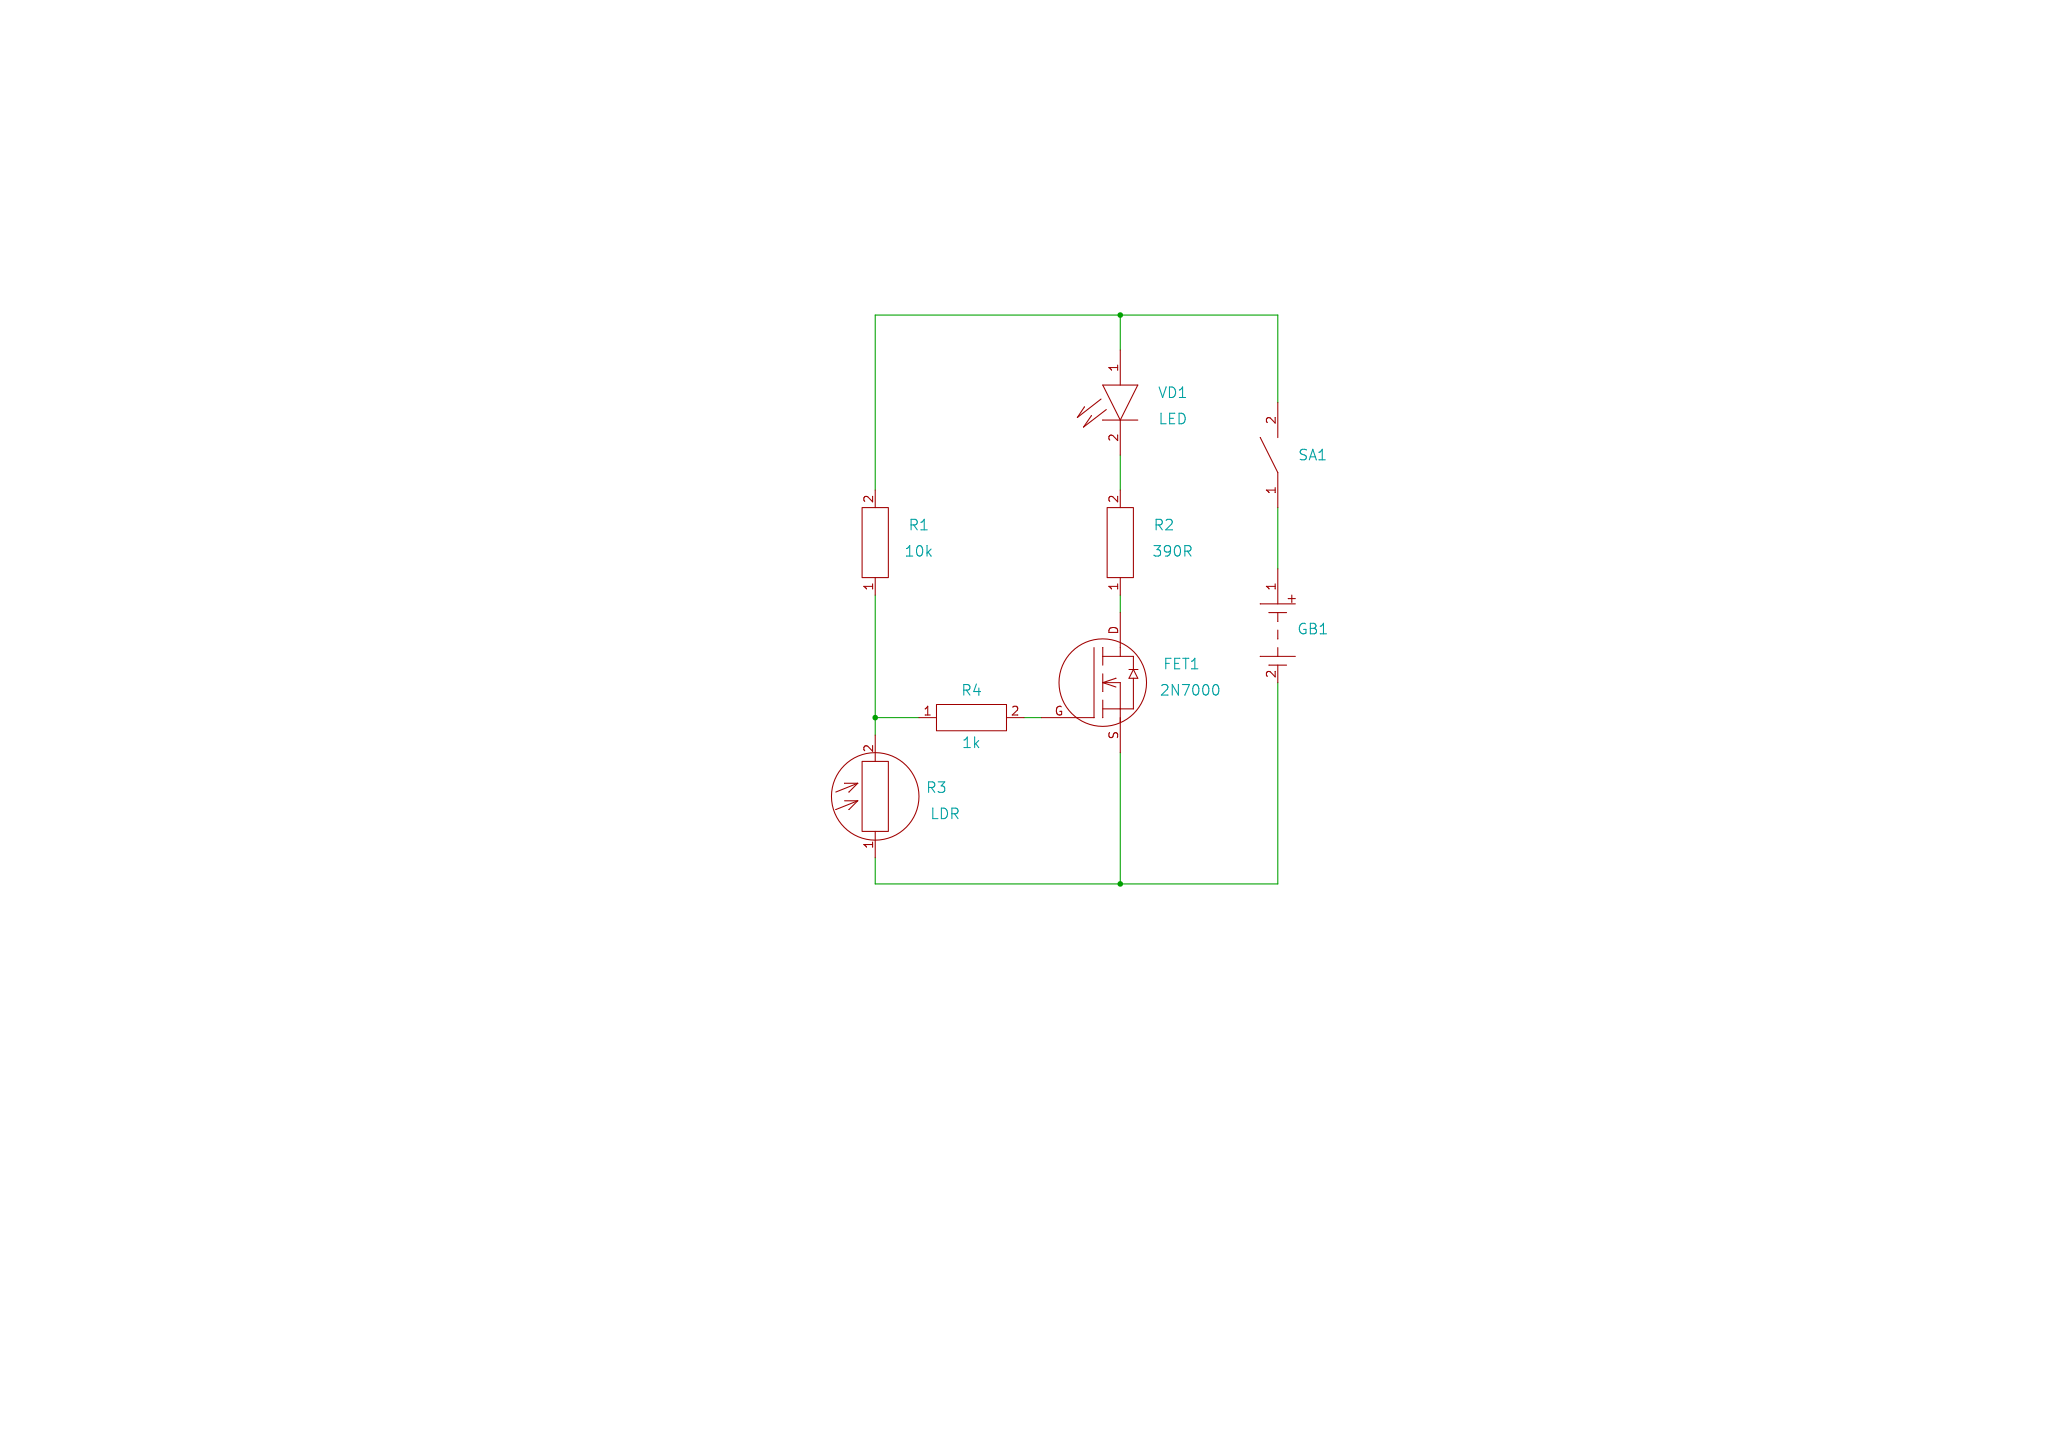
\includegraphics[height=0.65\textheight]{bcollis/ldr/ldr.pdf}
&\\
\end{tabular}
\bigskip

Компоненты на схеме: резистор R1 от 10K (10 000)\,Ом до 1M (1 000 000)\,Ом,
R3 фоторезистор, GB1 батарея. R1, R3\ --- схема делителя напряжения (питания),
резистор R2 ограничивает ток через светодиод VD1 и цепь исток/сток полевого
транзистора.

В темноте LDR имеет высокое сопротивление, и напряжение на выходе высокое.

На свету LDR имеет низкое сопротивление, и напряжение падает.

